%%%%%%%%%%%%%%%%%%%%%%%%%%%%%%%%%%%%%%%%%
% University Assignment Title Page 
% LaTeX Template
% Version 1.0 (27/12/12)
%
% This template has been downloaded from:
% http://www.LaTeXTemplates.com
%
% Original author:
% WikiBooks (http://en.wikibooks.org/wiki/LaTeX/Title_Creation)
%
% License:
% CC BY-NC-SA 3.0 (http://creativecommons.org/licenses/by-nc-sa/3.0/)
% 
% Instructions for using this template:
% This title page is capable of being compiled as is. This is not useful for 
% including it in another document. To do this, you have two options: 
%
% 1) Copy/paste everything between \begin{document} and \end{document} 
% starting at \begin{titlepage} and paste this into another LaTeX file where you 
% want your title page.
% OR
% 2) Remove everything outside the \begin{titlepage} and \end{titlepage} and 
% move this file to the same directory as the LaTeX file you wish to add it to. 
% Then add \input{./title_page_1.tex} to your LaTeX file where you want your
% title page.
%
%%%%%%%%%%%%%%%%%%%%%%%%%%%%%%%%%%%%%%%%%
%\title{Title page with logo}
%----------------------------------------------------------------------------------------
%	PACKAGES AND OTHER DOCUMENT CONFIGURATIONS
%----------------------------------------------------------------------------------------

\documentclass[12pt]{article}
\usepackage[english]{babel}
\usepackage[utf8x]{inputenc}
\usepackage{amsmath}
\usepackage{graphicx}
\usepackage[colorinlistoftodos]{todonotes}

% Custom packages
\usepackage{hyperref}
\usepackage{listings}
\usepackage[toc,page]{appendix}
\usepackage{pdfpages}
\usepackage{seqsplit}

%%
%% Julia definition (c) 2014 Jubobs
%%
\lstdefinelanguage{Julia}%
  {morekeywords={abstract,break,case,catch,const,continue,do,else,elseif,%
      end,export,false,for,function,immutable,import,importall,if,in,%
      macro,module,otherwise,quote,return,switch,true,try,type,typealias,%
      using,while},%
   sensitive=true,%
   alsoother={$},%
   morecomment=[l]\#,%
   morecomment=[n]{\#=}{=\#},%
   morestring=[s]{"}{"},%
   morestring=[m]{'}{'},%
}[keywords,comments,strings]%

\lstset{%
    language         = Julia,
    basicstyle       = \ttfamily\scriptsize,
    keywordstyle     = \bfseries\color{blue},
    stringstyle      = \color{magenta},
    commentstyle     = \color{ForestGreen},
    backgroundcolor  = \color{lightgray},
    showstringspaces = false,
    breaklines       = true,
    frame            = single
}

\begin{document}

\begin{titlepage}

\newcommand{\HRule}{\rule{\linewidth}{0.5mm}} % Defines a new command for the horizontal lines, change thickness here

\center % Center everything on the page
 
%----------------------------------------------------------------------------------------
%	HEADING SECTIONS
%----------------------------------------------------------------------------------------

\textsc{\Large Wroclaw University of Science and Technology}\\
\textsc{\large Faculty of Fundamental Problems of Technology}\\[2.5cm] % Minor heading such as course title\\[2.5cm] % Name of your university/college

%\textsc{\Large User Manual and Index}\\[1.0cm] % Major heading such as course name
%\textsc{\large Minor Heading}\\[0.5cm] % Minor heading such as course title

%----------------------------------------------------------------------------------------
%	TITLE SECTION
%----------------------------------------------------------------------------------------

\HRule \\[0.4cm]
{ \huge \bfseries{RobRecSolver package.\\ User Manual and API Reference}}\\[0.4cm] % Title of your document
\HRule

%----------------------------------------------------------------------------------------
%	REPORT SECTION
%----------------------------------------------------------------------------------------

Report: \textsc{Ser. PRE nr 3} \\[1.6cm]
 
%----------------------------------------------------------------------------------------
%	AUTHOR SECTION
%----------------------------------------------------------------------------------------

\begin{minipage}{1.0\textwidth}
\begin{flushright} \large
\emph{Author:} \\
Mikita \textsc{Hradovich}
\end{flushright}
\end{minipage}\\[2.5cm]

% If you don't want a supervisor, uncomment the two lines below and remove the section above
%\Large \emph{Author:}\\
%John \textsc{Smith}\\[3cm] % Your name

%----------------------------------------------------------------------------------------
%	DATE SECTION
%----------------------------------------------------------------------------------------

{\large 2019}\\[0.5cm] % Date, change the \today to a set date if you want to be precise

%----------------------------------------------------------------------------------------
%	LOGO SECTION
%----------------------------------------------------------------------------------------


\includegraphics[width=2.5cm]{logo.png} % Include a department/university logo - this will require the graphicx package
 
%----------------------------------------------------------------------------------------

\vfill % Fill the rest of the page with whitespace

\end{titlepage}

\tableofcontents{\protect\newpage}

\section{Introduction}

\href{https://github.com/nikagra/RobRecSolver.jl}{RobRecSolver} is a package written in a Julia programming language developed to test performance of algorithms proposed in M. Hradovich, A. Kasperski, P. Zieliński \textit{Robust recoverable 0-1 optimization problems under polyhedral uncertainty}\cite{DBLP:journals/corr/abs-1811-06719} 
which is available as preprint on \href{https://arxiv.org/abs/1811.06719}{arxiv.org}. This work was supported by the grant "Discrete optimization problems under uncertainty - models and algorithms" (2017/25/B/ST6/00486) by  the  National  Center  for  Science  (Narodowe
Centrum Nauki).

\subsection{Installing RobRecSolver}
If you are familiar with Julia you can quickly install RobRecSolver and CPLEX:
\begin{lstlisting}[language=Bash]
julia> Pkg.add("CPLEX")
julia> Pkg.clone("https://github.com/nikagra/RobRecSolver.jl.git")
\end{lstlisting}

\textbf{Note}: You need a working installation of CPLEX Optimizer. See \ref{sec:getting_cplex}{Getting CPLEX Optimizer} for more information.

\subsection{Citing}
You can cite \cite{DBLP:journals/corr/abs-1811-06719} by using the following BibTeX snippet:
\begin{lstlisting}{language=LaTeX}
@article{hradovich2018robust,
  title={Robust recoverable 0-1 optimization problems under polyhedral uncertainty},
  author={Hradovich, Mikita and Kasperski, Adam and Zielinski, Pawel},
  journal={arXiv preprint arXiv:1811.06719},
  year={2018}
}   
\end{lstlisting}

\section{Instalation Guide}
This guide will briefly guide you through installing Julia, CPLEX Optimizer and RobRecSolver with all of its dependencies.

\subsection{Getting Julia}
Version of Julia programming language required by JuMP and consequently by RobRecSolver is \texttt{0.6}. You can build Julia from source or use the binaries.

Download links and more detailed instructions are available on the \href{https://julialang.org/downloads/}{Julia} website.

\subsection{Getting CPLEX Optimizer}
\label{sec:getting_cplex}
RobRecSolver package depends on \href{https://github.com/JuliaOpt/CPLEX.jl}{CPLEX.jl} which in turn requires a working installation of \href{https://www.ibm.com/analytics/cplex-optimizer}{CPLEX Optimizer} with a license, which is free for faculty members and graduate teaching assistants.

CPLEX Optimizer must be downloaded and installed separately. Check \href{https://github.com/JuliaOpt/CPLEX.jl}{CPLEX.jl} for further instructions.

\subsection{Getting RobRecSolver}
RobRecSolver package is \textit{not} yet registered in the \href{https://github.com/JuliaLang/METADATA.jl}{METADATA.jl} repository. To install it, use \texttt{Pkg.clone} command:
\begin{lstlisting}
julia> Pkg.clone("https://github.com/nikagra/RobRecSolver.jl.git")
\end{lstlisting}

Since RobRecSolver contains REQUIRE file, that file will be used to determine which
registered packages RobRecSolver depends on, and they will be automatically installed.

\subsection{Updating RobRecSolver}
In order to update package run the following sequence of commands (\texttt{;} symbol
at the start of the Julia's REPL enters shell mode):
\begin{lstlisting}
julia> cd(Pkg.dir("RobRecSolver"))
julia> ;
shell> git fetch --all --tags --prune && git checkout tags/<version>
julia> Pkg.resolve()
\end{lstlisting}
You may want to check \href{https://git-scm.com/book/en/v2}{Pro Git} written by Scott Chacon and Ben Straub to learn more about git version control system.

\section{Manual}

\subsection{Getting Started}
Package consists of a number of functions implementing algorithms described in \cite{DBLP:journals/corr/abs-1811-06719} as well as some utility functions. The easiest way to experiment with them is to use package in Julia's interactive session (or REPL which stands for read-eval-print loop). For example:
\begin{lstlisting}{language=Julia}
$ julia
               _
   _       _ _(_)_     |  A fresh approach to technical computing
  (_)     | (_) (_)    |  Documentation: https://docs.julialang.org
   _ _   _| |_  __ _   |  Type "?help" for help.
  | | | | | | |/ _` |  |
  | | |_| | | | (_| |  |  Version 0.6.3 (2018-05-28 20:20 UTC)
 _/ |\__'_|_|_|\__'_|  |  Official http://julialang.org/ release
|__/                   |  x86_64-w64-mingw32

julia> 1 + 1
2
\end{lstlisting}

Interactive session may be useful while prototyping programs since it outputs result of each evaluation and allows to check intermediate results.

To leave interactive session enter \texttt{exit()} command or press \texttt{Ctrl+D}.

Alternatively you can evaluate source file, which uses \texttt{.jl} filename extension by convention:

\begin{lstlisting}{language=Bash}
$ julia main.jl arg
\end{lstlisting}

In the example above Julia passes argument \texttt{arg} to the program stored in source file named \texttt{main.jl} and then execute commands stored in it in non-interactive mode. Arguments passed to program are available within script in a global constant \texttt{ARGS}, thus name of the source file in global constant \texttt{PROGRAM\_FILE}.

See \href{https://docs.julialang.org/en/v1/manual/faq/#man-scripting-1}{Julia Scripting} for more information about writing scripts in Julia.

To start using RobRecSolver library first import it, some of its submodules or functions with \texttt{using} keyword, then call function you are interested in, i.e. \texttt{incrementalProblem}:
\begin{lstlisting}{language=Bash}
julia> using RobRecSolver.Experiments
julia> runExperiments([100, 400, 1000], [10, 25, 100])
\end{lstlisting}
Check \href{https://docs.julialang.org/en/v0.6/manual/modules/#modules-1}{Julia Modules} for more detailed information about using modules in Julia.


\subsection{Additional Types and Functions}
There is a number of types and helper functions defined to facilitate implementation of algorithms described in \cite{DBLP:journals/corr/abs-1811-06719}. \texttt{ProblemDescriptor} is one of such a types. It serves as a basic interface, defining size of the problem or whether it has equal cardinality property among other properties. There two subtypes of \texttt{ProblemDescriptor}, namely \texttt{KnapsackProblemDescriptor} and \texttt{AssignmentProblemDescriptor} for each problem discussed in \cite{DBLP:journals/corr/abs-1811-06719}:
\begin{lstlisting}{language=Julia}

using RobRecSolver

n = 5
knapsackProblemDescriptor = KnapsackProblemDescriptor(n)
property = hasEqualCardinalityProperty(knapsackProblemDescriptor)
println("KnapsackProblemDescriptor.hasEqualCardinalityProperty: $property")

assignmentProblemDescriptor = AssignmentProblemDescriptor(n)
property = hasEqualCardinalityProperty(assignmentProblemDescriptor)
println("AssignmentProblemDescriptor.hasEqualCardinalityProperty: $property")
println("AssignmentProblemDescriptor.getCardinality: $(getCardinality(assignmentProblemDescriptor))")

\end{lstlisting}
Upon executing example above you will get the following output:
\begin{lstlisting}
KnapsackProblemDescriptor.hasEqualCardinalityProperty: false
AssignmentProblemDescriptor.hasEqualCardinalityProperty: true
AssignmentProblemDescriptor.getCardinality: 5
\end{lstlisting}

Function \texttt{initialScenario} is another example of a helper function. It searches for good heuristic initial scenario in order to speed up some computations. Its behavior is described in the section 5.1 \textit{Adversarial lower bound} of \cite{DBLP:journals/corr/abs-1811-06719}. See example below on how to use this function:
\begin{lstlisting}[mathescape]{language=Julia}
using RobRecSolver

c = [2, 3]
d = [8, 9]
$\Gamma$ = 10
s = initialScenario(c, d, $\Gamma$)
println("Initial scenario is ", s)
\end{lstlisting}

In this example \texttt{c} is a vector of second stage costs, \texttt{d} is vector of maximal deviations of the costs from their nominal values and \texttt{$\Gamma$} is a budget or the amount of uncertainty, which can be allocated to the second stage costs.

Upon running the script above you will receive the following output:
\begin{lstlisting}{language=Julia}
Initial scenario is [7.50073, 7.50073]
\end{lstlisting}

The functions \texttt{loadProperties} and \texttt{getProperty} allow to customize package parameters like solver time limits or logging for different algorithms.

Function \texttt{loadProperties} loads properties stored in an INI file from the specified file location. To change default location set \texttt{ROBRECSOLVER\_CONFIG} environment variable either in Julia REPL or in \texttt{~/.julia/config/startup.jl} and then reload RobRecSolver package:
\begin{lstlisting}{language=Julia}
julia> ENV["ROBRECSOLVER_CONFIG"] = "<path_to_file>"
julia> Pkg.reload("RobRecSolver")
\end{lstlisting}
Use default properties file \texttt{Pkg.dir("RobRecSolver")/conf/config.ini} as a reference. Below is an extract from it:
\begin{lstlisting}
; Problem properties
[main]
lagrangianLowerBound.cplexLogging=0
lagrangianLowerBound.epsilon=0.000001
lagrangianLowerBound.overallTimeLimit=1800
lagrangianLowerBound.subproblemTimeLimit=600
\end{lstlisting}
See Appendix~\ref{sec:properties} for full contents.

In order to reset changes simply delete environment variable and reload RobRecSolver package.

Function \texttt{getProperty} returns value for key from previously loaded properties file:
\begin{lstlisting}[mathescape]{language=Julia}
using RobRecSolver

$\epsilon$ = getProperty("evaluationProblem.epsilon", parameterType = Float64)
timeLimit = getProperty("evaluationProblem.timeLimit")
\end{lstlisting}
In the example above value for property \texttt{evaluationProblem.epsilon} of type \texttt{Float64} is stored in variable \texttt{$\epsilon$}. Then value for property \texttt{\seqsplit{evaluationProblem.timeLimit}} of type \texttt{Int} (default) is stored in variable \texttt{timeLimit}. If properties section is not specified, section called \texttt{main} is used by default.

\section{Problems}
\subsection{Incremental and Recoverable Problems}
Section 4 \textit{Solving the problems by MIP formulations} of \cite{DBLP:journals/corr/abs-1811-06719} presents MIP formulations for incremental and recoverable problems for element exclusion neighborhood as well its simplified versions for equal cardinality problem.

Both versions of incremental problems are solved by \texttt{incrementalProblem} function. Here is example of solving incremental problem for minimum knapsack problem:
\begin{lstlisting}[mathescape]{language=Julia}
julia> using RobRecSolver
julia> n = 3
julia> $\alpha$ = 0.5
julia> c = [1, 2, 3]
julia> x = [0, 1, 1]
julia> w = [1, 2, 2]
julia> W = 3
julia> X = getKnapsackConstraints(w, W)
julia> problemDescriptor = KnapsackProblemDescriptor(n)
julia> incrementalProblem(c, $\alpha$, x, X, problemDescriptor)
\end{lstlisting}
In this example we first import RobRecSolver package. Then we define a number of variables, namely \texttt{c} for a vector of nonnegative nominal second stage costs, \texttt{x} for a first stage solution, variable \texttt{$\alpha$} for fixed number belonging to \texttt{[0,1]} as described in \cite{DBLP:journals/corr/abs-1811-06719}. We also define variable \texttt{w} for a vector of item weights and \texttt{W} for knapsack capacity. Set of feasible solutions is prepared by function \texttt{getKnapsackConstraints}. It is represented as a list of anonymous functions each of which for given vector of JuMP variables returns a JuMP linear constraint. Variable \texttt{problemDescriptor} is an instance of type \texttt{KnapsackProblemDescriptor} which defines some useful properties of a problem, i.e. its size or whether it has equal cardinality property. Last step is to call function \texttt{incrementalProblem}. It will return tuple containing vector of second stage solutions and objective value.

Let us solve recoverable problem for minimum assignment problem using \texttt{recoverableProblem} function:
\begin{lstlisting}[mathescape]{language=Julia}
julia> using RobRecSolver
julia> m = 2
julia> $\alpha$ = 1.0
julia> C = [1 2; 3 1]
julia> c = [5 3; 2 4]
julia> X = getAssignmentConstraints(m)
julia> problemDescriptor = AssignmentProblemDescriptor(m)
julia> recoverableProblem(C, c, X, $\alpha$, problemDescriptor)
\end{lstlisting}
As in a previous example we first define some auxiliary variables. Here  \texttt{C} is a vector of nonnegative first stage costs,  \texttt{C} is a vector of a nonnegative nominal second stage costs, \texttt{X} is a set of feasible solutions,  \texttt{$\alpha$} is fixed number belonging to \texttt{[0, 1]} and \texttt{problemDescriptor} is an instance of \texttt{\seqsplit{AssignmentProblemDescriptor}}. This example will return a tuple consisting of a vector of first stage solutions, a vector of second stage solutions and objective value.

\subsection{Evaluation Problem}
Let us take a look at a function named \texttt{evaluationProblem}, which implements \textbf{Algorithm 1} of Section 4 \textit{Solving the problems by MIP formulations} of \cite{DBLP:journals/corr/abs-1811-06719}. Here is an example of how one can use it for minimum knapsack problem:
\begin{lstlisting}[mathescape]{language=Julia}
julia> using RobRecSolver
julia> n = 2
julia> $\alpha$ = 1.0
julia> C = [4, 3]
julia> c = [2, 3]
julia> d = [8, 9]
julia> $\Gamma$ = 9
julia> x = [0, 1]
julia> w = [1, 2]
julia> W = 1
julia> X = getKnapsackConstraints(w, W)
julia> problemDescriptor = KnapsackProblemDescriptor(n)
julia> evaluationProblem(C, c, d, $\Gamma$, $\alpha$, x, X, problemDescriptor)
D-  2 constraints was added to this evaluation problem                 Debug evaluation_problem.jl:1
10.0
\end{lstlisting}
We first define size of a problem \texttt{n}, parameter  \texttt{$\alpha$}, a vector of first stage costs  \texttt{C}, a vector of a nonnegative nominal second stage costs  \texttt{C}, a vector of maximal deviations of the costs from their nominal values  \texttt{d}, budget  \texttt{$\Gamma$}, set of feasible solutions \texttt{X} and an instance of type \texttt{KnapsackProblemDescriptor} \texttt{problemDescriptor}. We also define a vector of item weights \texttt{w} and knapsack capacity \texttt{w}. The last step is to call \texttt{evaluationProblem} passing all necessary arguments.

\subsection{Lower Bounds}
Section 5 \textit{Lower bounds} of the publication contains algorithms and MIP formulations to calculate adversarial, lagrangian and cardinality selection constraint lower bounds. Corresponding functions from RobRecSolver package to calculate this lower bounds are respectively \texttt{adversarialProblem}, \texttt{lagrangianLowerBound} and \texttt{selectionLowerBound}. All of this function have very similar signatures, so as an example let us take a closer look to \texttt{adversarialProblem}. This function implements algorithm for calculating adversarial lower bound shown in the form of \textbf{Algorithm 2} of Section 5.1 \textit{Solving the problems by MIP formulations} of the publication. Below is an example of source file solving it for minimum knapsack problem saved as \texttt{adv.jl}:
\begin{lstlisting}[mathescape]{language=Julia}
using RobRecSolver

n = 2
$\alpha$ = 0.5

w = [1, 2]
W = 1
X = getKnapsackConstraints(w, W)

C = [1, 3]
c = [3, 1]
d = [2, 2]
$\Gamma$ = 2

problemDescriptor = KnapsackProblemDescriptor(n)
result = adversarialProblem(C, c, d, $\Gamma$, X, $\alpha$, problemDescriptor)
println("Adversarial lower bound is ", result)
\end{lstlisting}
Assuming the above code is saved as \texttt{adv.jl}, running the above program will return the following output:
\begin{lstlisting}{language=Julia}
$ julia adv.jl
D-  3 constraints was added to this adversarial problem               Debug adversarial_problem.jl:1
Adversarial lower bound is 5.0
\end{lstlisting}
In this program we first define size of a problem \texttt{n}, parameter  \texttt{$\alpha$}, a vector of first stage costs  \texttt{C}, a vector of a second stage costs  \texttt{C}, a vector of maximal deviations of the costs from their nominal values  \texttt{d}, budget  \texttt{$\Gamma$}, set of feasible solutions \texttt{X} and an instance of type `KnapsackProblemDescriptor` `problemDescriptor` defining problem properties. Then we call `adversarialProblem` function passing all necessary arguments and printing out result. Note, that depending on package settings it also may print some additional logs.

\subsection{Experiments}
RobRecSolver package also contains \texttt{Experiments} submodule which can serve as a reference on how to use core package functionality in experiments. Please remember that almost all functions in \texttt{RobRecSolver.Experiments} are highly customized to serve purposes of \cite{DBLP:journals/corr/abs-1811-06719}. Never the less let us take a closer look at functions presented here.

\texttt{RobRecSolver.Experiments.runExperiments} is an entry point of experiments. It accepts list of minimum knapsack problem sizes \texttt{ns}, list of minimum assignment problem sizes \texttt{ms} and optionally list of values of parameter $\alpha$ called \texttt{$\alpha$s} and a number of instances to be generated for each value of $\alpha$ called \texttt{numberOfInstances}. By default \texttt{$\alpha$s} has values $0.1,0.2,...,0.9$ and \texttt{numberOfInstances} equals 5:
\begin{lstlisting}[mathescape]{language=Julia}
using RobRecSolver.Experiments

runExperiments([100, 400, 1000], [10, 25, 100])
\end{lstlisting}
Check \cite{DBLP:journals/corr/abs-1811-06719} for more information about scope of experiments.

\texttt{RobRecSolver.Experiments.saveCsv} is a helper function developed to save experiment results as CSV files. It saves data described by \texttt{columnNames} argument using data passed in \texttt{data} argument to CSV file with name \texttt{filename}:
\begin{lstlisting}[mathescape]{language=Julia}
using RobRecSolver

Experiments.saveCsv("item_prices.csv", ["milk" 100; "ham" 250], ["item", "price"])
\end{lstlisting}
The above program will save CSV file \texttt{item\_prices.csv} with the following content:
\begin{lstlisting}{language=CSV}
item,price
milk,100
ham,250
\end{lstlisting}

Function \texttt{RobRecSolver.Experiments.drawAndSavePlot} is a function used to draw plots used in \cite{DBLP:journals/corr/abs-1811-06719}. It accepts a number of parameteres and is heavily based on \texttt{PyPlot} backend. As an example. the following code snippet:
\begin{lstlisting}[mathescape]{language=Julia}
using RobRecSolver, Plots

pyplot()
Experiments.drawAndSavePlot("plot.pdf", [0.1, 0.2, 0.3], [21, 15, 12], "$\alpha$", "average time (s)", "m=100")
\end{lstlisting}
Will produce the following plot:

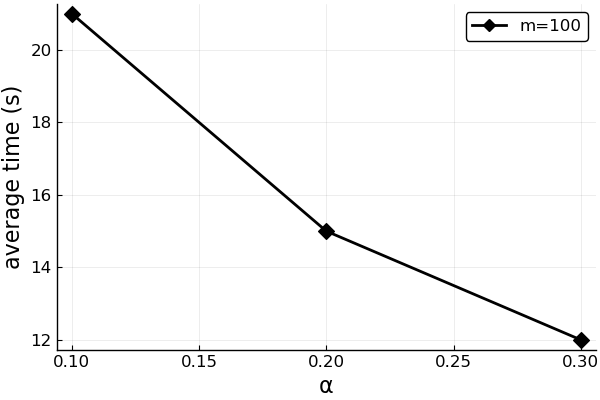
\includegraphics[width=\textwidth]{plot.png}

Check the Appendix A.2 for more complete reference of functions used in experiments.

\section{Acknowledgements}
This work was supported by the National Center for Science (Narodowe Centrum Nauki), grant 2017/25/B/ST6/00486.

\clearpage
\appendix
\section{Appendices}

\subsection{Properties File}
\label{sec:properties}
\begin{lstlisting}
; Problem properties
[main]
lagrangianLowerBound.cplexLogging=0
lagrangianLowerBound.epsilon=0.000001
lagrangianLowerBound.overallTimeLimit=1800
lagrangianLowerBound.subproblemTimeLimit=600

selectionLowerBound.timeLimit=600
selectionLowerBound.cplexLogging=0

adversarialProblem.timeLimit=600
adversarialProblem.cplexLogging=0
adversarialProblem.epsilon=0.01

evaluationProblem.timeLimit=600
evaluationProblem.cplexLogging=0
evaluationProblem.epsilon=0.01

incrementalProblem.cplexLogging=0

minimumAssignmentProblem.cplexLogging=0

minimumKnapsackProblem.cplexLogging=0

recoverableProblem.cplexLogging=0
\end{lstlisting}
\clearpage

%\subsection[subsectionstyle=hide]{Reference}
\addcontentsline{toc}{subsection}{A.2\hspace{3 mm}Reference}
\setcounter{subsection}{+1}
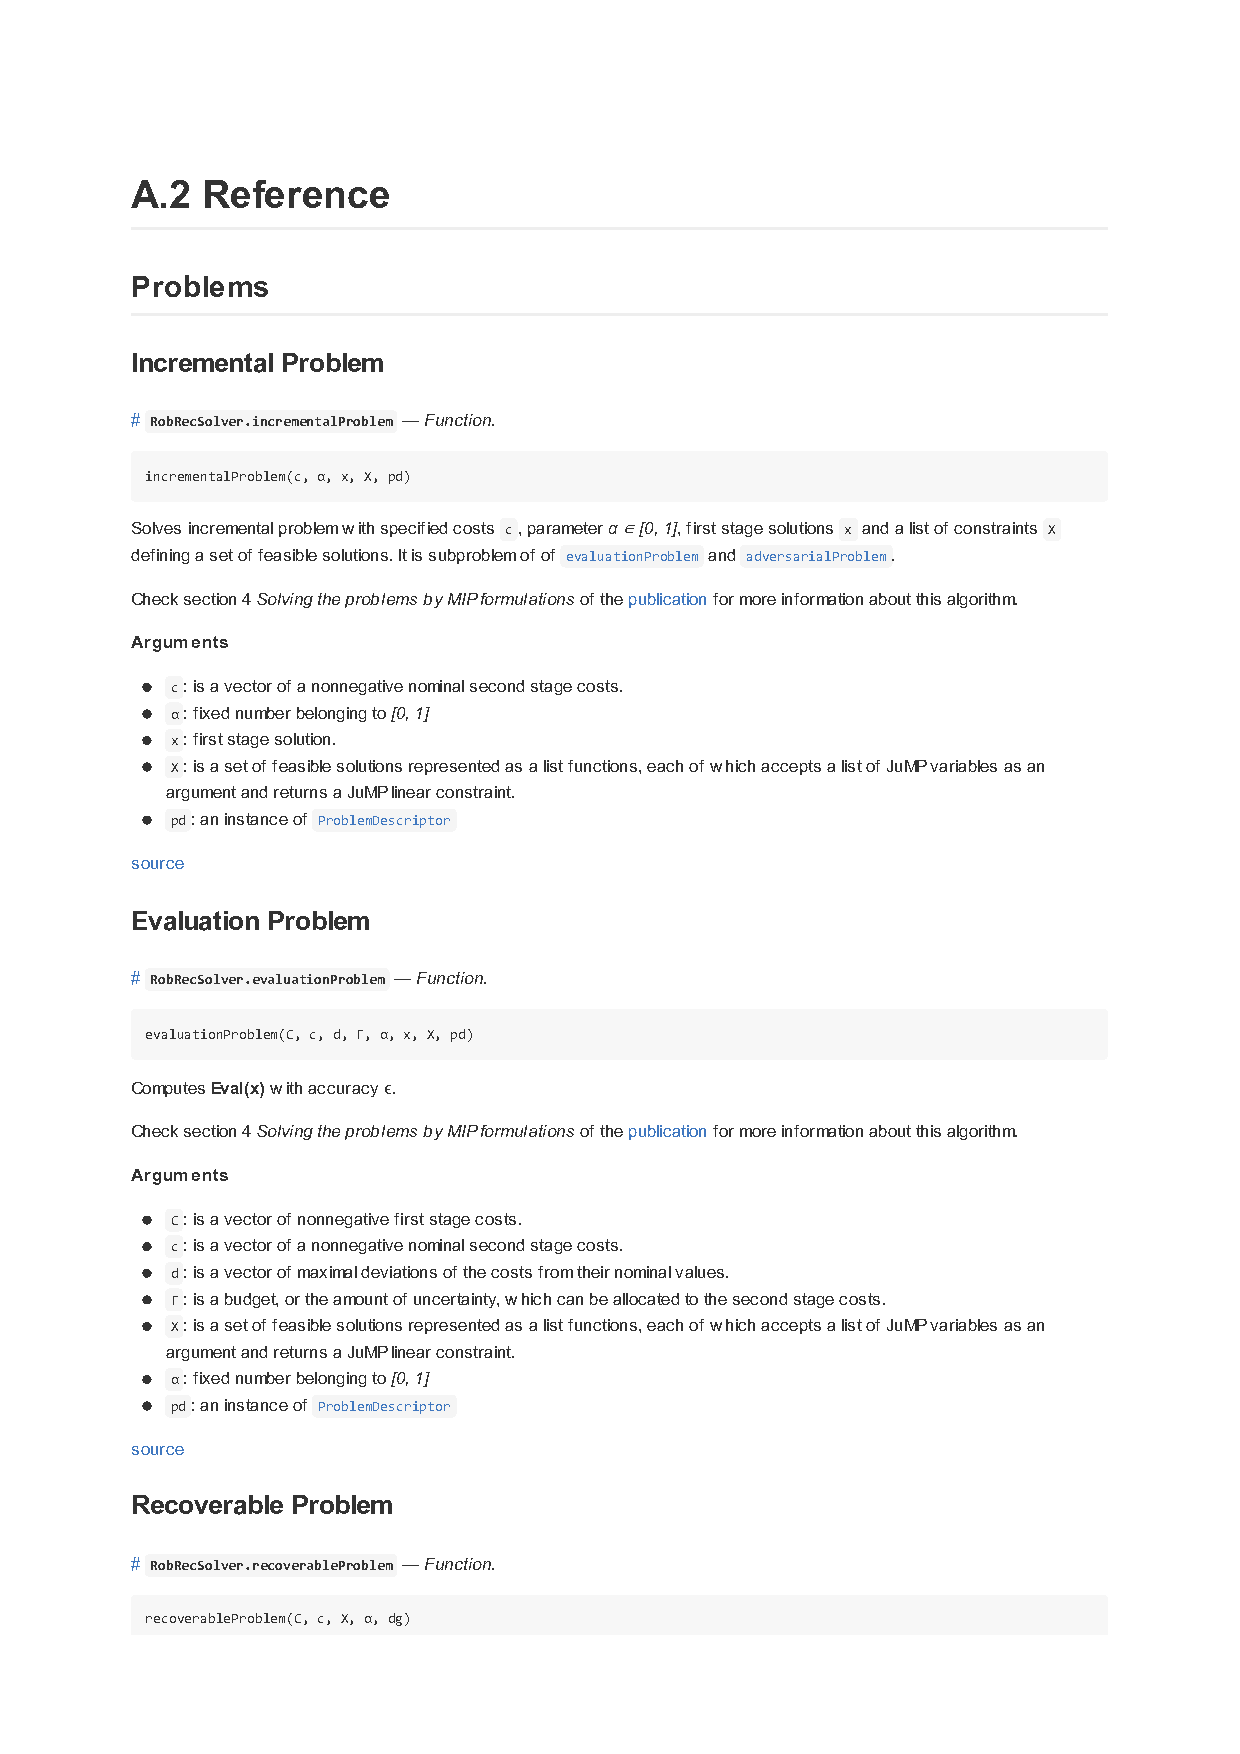
\includepdf[pages=-]{reference.pdf}

\bibliography{bibliography}{}
\bibliographystyle{plain}

\end{document}